\input{configuration}

\title{Lecture 27 --- File System Implementation and Allocation Methods}

\author{Jeff Zarnett \\ \small \texttt{jzarnett@uwaterloo.ca}}
\institute{Department of Electrical and Computer Engineering \\
  University of Waterloo}
\date{\today}


\begin{document}

\begin{frame}
  \titlepage

 \end{frame}




\begin{frame}
\frametitle{Virtual File System}

There are a lot of different file systems, like ext3, ZFS... 

These may co-exist in a system, though a partition will be formatted in only one.

From the user's perspective, however, these operate identically. 

This is because of an additional layer of abstraction: virtual file system (VFS). 

\end{frame}

\begin{frame}
\frametitle{Virtual File System}

There are two main purposes to the VFS. 

The first is to separate the file system operations (like reading, writing, opening, and closing files) from the actual implementation. 

Thus operations can be done with whatever file system is implemented. 

The second is that it provides a mechanism for representing a file, uniquely, throughout a network. 

The file representation structure is called a \textit{vnode}, which is rather like an inode, but inodes are unique only within one file system. 

The VFS distinguishes between local and remote files.

\end{frame}

\begin{frame}
\frametitle{Virtual File System}

\begin{center}
	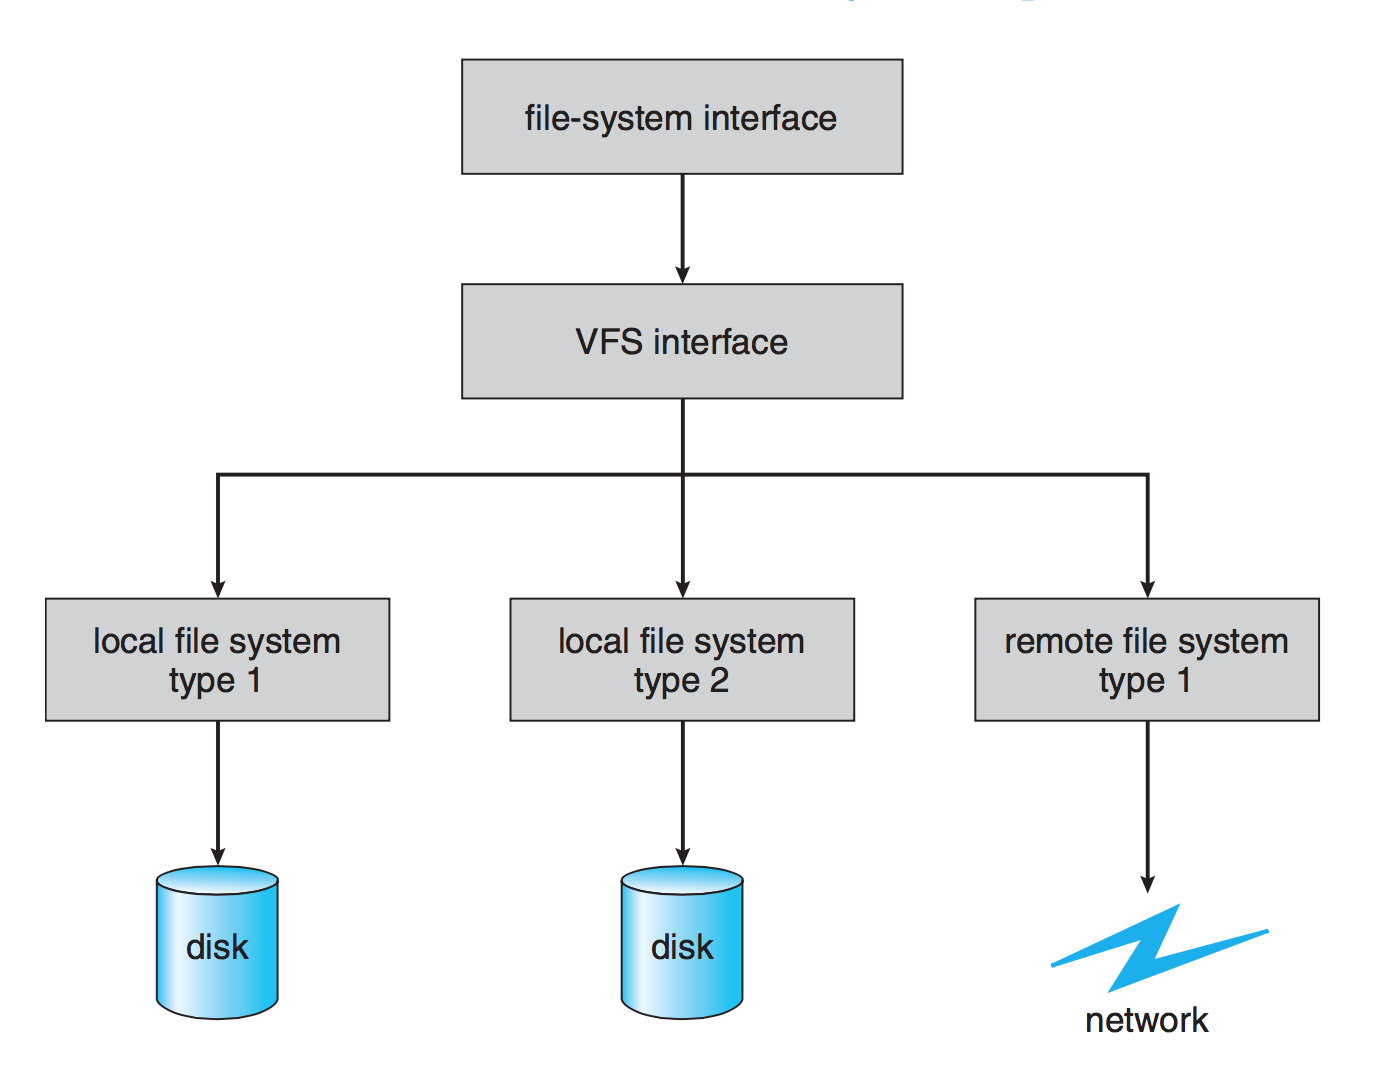
\includegraphics[width=0.85\textwidth]{images/vfs.png}
\end{center}


\end{frame}

\begin{frame}
\frametitle{Virtual File System}

The VFS architecture in Linux has four main objects:

\begin{enumerate}
	\item inode (an individual file)
	\item file (an open file)
	\item superblock (the file system)
	\item dentry (a directory entry)
\end{enumerate}



\end{frame}

\begin{frame}[fragile]
\frametitle{Virtual File System}

For each of those, there are a set of operations defined. 

On a file, for example:
{\scriptsize
\begin{verbatim}
 ssize_t (*read) (struct file *, char __user *, size_t, loff_t *);
 ssize_t (*write) (struct file *, const char __user *, size_t, loff_t *); 
 int (*open) (struct inode *, struct file *);
 int (*flush) (struct file *, fl_owner_t id);
 int (*release) (struct inode *, struct file *);
\end{verbatim}
}

\end{frame}

\begin{frame}
\frametitle{Directory Implementation}

\begin{center}
	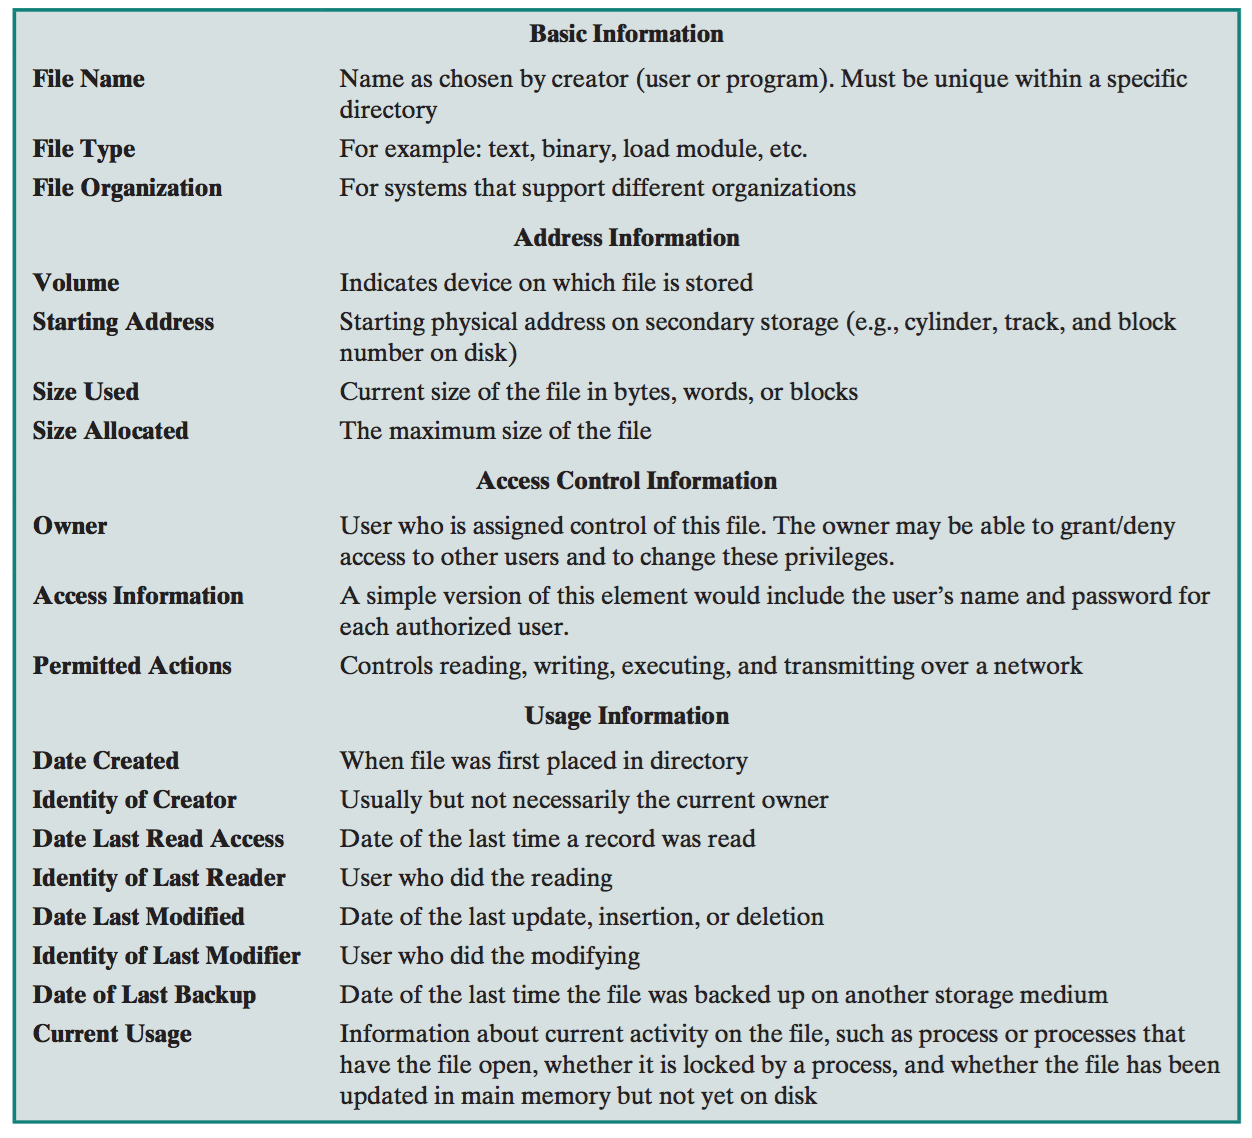
\includegraphics[width=0.75\textwidth]{images/directory.png}
\end{center}

\end{frame}



\begin{frame}
\frametitle{Directory Implementation}

A directory is, after all, not much beyond a set of files. 

And yet, there is a choice to be made in implementing them.

A linear list versus a hash table? 

Both concepts should be familiar to you from data structures and algorithms.


\end{frame}

\begin{frame}
\frametitle{Directory Implementation}

The linear list option is certainly the simplest. 

Creating a new file: search the directory to see if there is a matching file name. 

If not, insert that new entry in the list. 

Deletion is also simple: search the list for the matching file and remove it; if it is the last reference to that file, we can free up the space. 

The real disadvantage to linear lists is that searching takes a long time. 

Searching through a directory can take quite a while.

\end{frame}

\begin{frame}
\frametitle{Directory Implementation}

Alternatively, we could use a hash table. 

The hash is computed based on the file name, and of course there will need to be some strategy for dealing with hash collisions. 

Still, neither of these is satisfactory. 

What we really want is a more complex structure: a tree.


\end{frame}

\begin{frame}
\frametitle{AVL and B-Trees}


An AVL tree might be good as a way of storing ordered data. 

It does not match well with the block system of a hard drive. 

Instead, we will examine a B-Tree, a balanced, ordered tree.


\end{frame}

\begin{frame}
\frametitle{B-Tree}

Each node should occupy one block, so each node can contain a lot of info. 

File \& directory info is linearly ordered, but a block does not need to be full. 

If a leaf node gets full, we can split it into two half-full blocks. 

Keeping the tree balanced means it takes about the same amount of time to find an item wherever it is.


\end{frame}

\begin{frame}
\frametitle{B-Tree Structure}

A B-Tree structure, formally, has the following characteristics:

\begin{enumerate}
	\item The tree is made up of nodes (have children) and leaves (have no children).
	\item Each node contains at least one key identifying a file record, and more than one pointer to child nodes or child leaves.
	\item Each node has some maximum number of keys.
	\item The keys in a node are stored in non-decreasing order.
\end{enumerate}

\end{frame}



\begin{frame}
\frametitle{B-Tree Properties}

Properties of the B-Tree:

\begin{enumerate}
	\item Every node has at most $2d-1$ keys and $2d$ children ($2d$ pointers).
	\item Every node other than the root has at least $d-1$ keys and $d$ pointers. Each internal node except the root is at least half full and has at least $d$ children.
	\item All leaves appear on the same level.
	\item A non-leaf node with $k$ pointers contains $k-1$ keys.
\end{enumerate}

\end{frame}

\begin{frame}
\frametitle{Searching a B-Tree}

To find something in a B-Tree, the general algorithm is fairly simple:

\begin{enumerate}
	\item Start at the root node. 
	\item If the key is in the current node, it is found, and the algorithm terminates.
	\item If the key is less than the smallest key in this node, follow the leftmost pointer; go to step 2.
	\item If the key is greater than the largest key in this node, follow the rightmost pointer; go to step 2.
	\item If the key is between the values of two adjacent keys, follow the pointer between them; go to step 2.
\end{enumerate}



\end{frame}

\begin{frame}
\frametitle{B-Tree Insertion}

Insertion into the B-Tree is more complicated:

\begin{enumerate}
	\item Search the tree for the key. If it is not found, then we are at least looking at the block where it would be if it were there.
	\item If this node has fewer than $2d-1$ keys (that is, it is not full), insert the key into this node in the proper sequence. The algorithm terminates.
	\item If the node is full, split this node around the median key into two new nodes with $d-1$ keys each. Promote the median key to the higher level. If the new key is less than the median key, insert it in the left-hand new node; otherwise into the right.
	\item The promoted key is inserted into the parent node in order, splitting the parent if the parent is already full.
	\item If the process of promotion reaches the root node and the root is full, then splitting and promotion occurs and the height of the tree increases by 1.
\end{enumerate}


\end{frame}



\begin{frame}
\frametitle{B-Tree Operations}


\begin{center}
	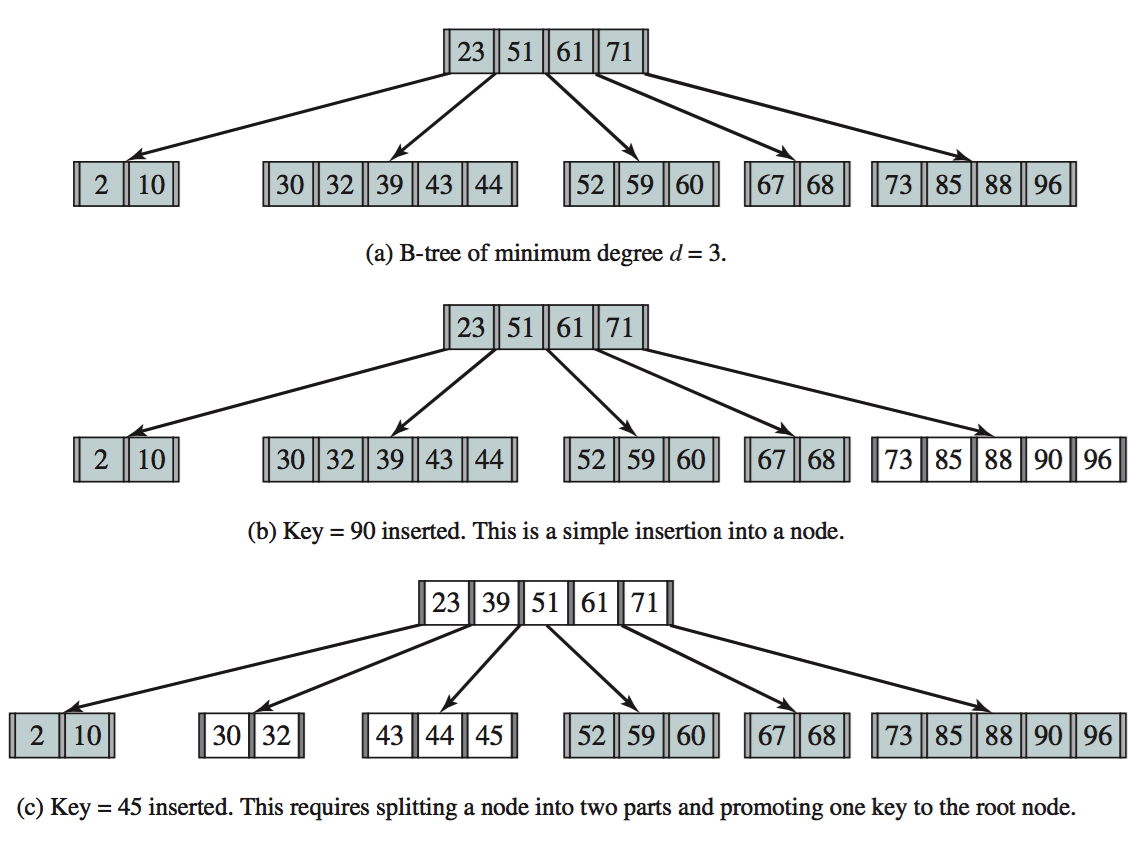
\includegraphics[width=0.9\textwidth]{images/b-tree-insert-top.png}
\end{center}


\end{frame}

\begin{frame}
\frametitle{B-Tree Operations}


\begin{center}
	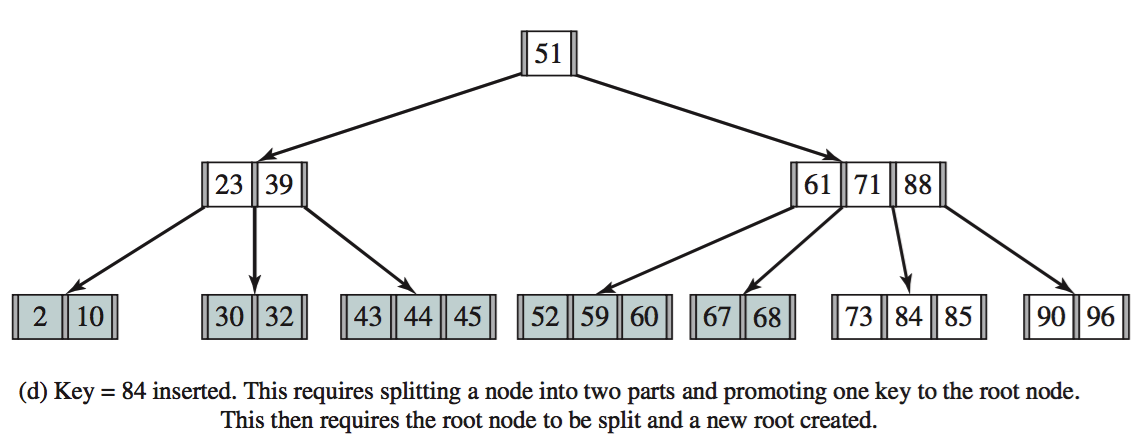
\includegraphics[width=0.9\textwidth]{images/b-tree-insert-bottom.png}
\end{center}


\end{frame}

\begin{frame}
\frametitle{Allocation of Disk Space}

There is a need to choose a strategy for how to allocate disk space. 

\begin{center}
	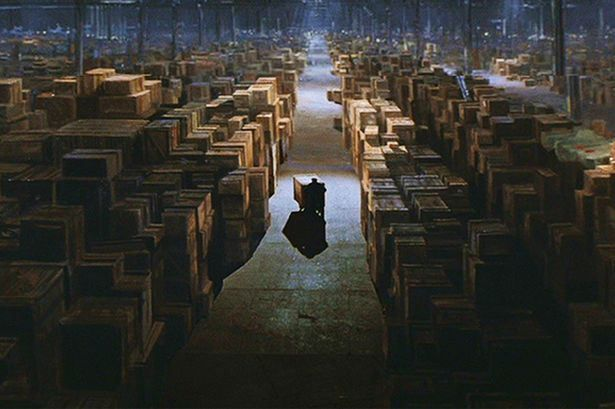
\includegraphics[width=0.4\textwidth]{images/jones.jpg}
\end{center}

There are three major ways that we could allocate the disk space to files:\\
\quad Contiguous, linked, and indexed; each has its advantages and disadvantages.


\end{frame}

\begin{frame}
\frametitle{Contiguous Allocation}
Contiguous: a file occupies a set of contiguous blocks on disk. 

So if a file is allocated, starting at block $b$ and is $n$ blocks in size, the file takes up blocks $b, b+1, b+2, ..., b+(n-1)$. 

This is advantageous, because if we want to access block $b$ on disk, accessing $b+1$ requires no head movement, so seek time is nonexistent to minimal.

\end{frame}

\begin{frame}
\frametitle{Contiguous Allocation}

All that we need to maintain are $b$ and $n$: the start location and length of the file. 

Both sequential and direct access are very easy: the first block of a file is at $b$. 

To access a block $i$ at some offset into the file, it's at the base address $b$ plus $i$. 

Checking if the access is valid is also an easy operation: if $i < n$ then it is valid.

\end{frame}

\begin{frame}
\frametitle{Contiguous Allocation}

\begin{center}
	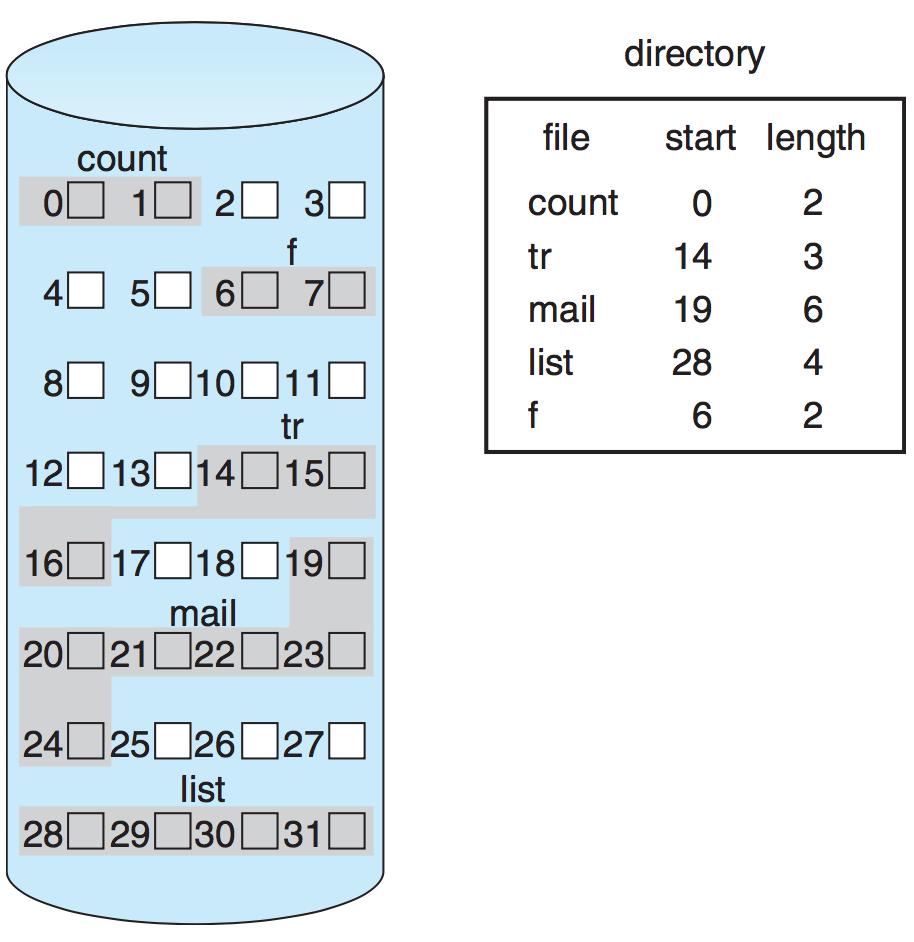
\includegraphics[width=0.6\textwidth]{images/disk-contiguous.png}
\end{center}

\end{frame}

\begin{frame}
\frametitle{Contiguous Allocation}

This takes us back to a problem we have seen once before: the memory allocation problem. 

If we need a memory block of size $N$:\\
\quad (1) can we find a contiguous block of $N$ or greater to meet that allocation?\\
\quad (2) if there is more than one block, which one do we choose? 

As before, we suffer the problem of external fragmentation, plus a bit of internal fragmentation in the last block of the file. 

\end{frame}

\begin{frame}
\frametitle{Contiguous Allocation and Compaction}

There was also talk on the subject of memory allocation of compaction. 

This was moving memory allocations around in memory to create some larger free spaces that can be allocated. 

But for languages like C, it was not realistic, because of the impossibility of updating all pointers (unlike Java where we can update all references). 

\end{frame}

\begin{frame}
\frametitle{Compaction}

We can do compaction on disk, but it's slow and computationally expensive. 

Doing compaction can be done when the system has nothing else to do (idle priority operation) or on some schedule when it would be minimally disruptive.

The middle of the night...?


\end{frame}

\begin{frame}
\frametitle{Contiguous Allocation}

Another problem: how much space is a file going to take? 

If it is just a copy-paste operation, the copy is the same size as the original. 

When a user opens a new document, how big will it be? 

\end{frame}

\begin{frame}
\frametitle{Contiguous Allocation}


If we allocate too little space, we may be able to tack on space at the end, or that block may be allocated, forcing us to move the file and reallocate it. 

If the value we choose is too large, then significant space will be wasted for small files (and many files tend to be relatively small).

\end{frame}

\begin{frame}
\frametitle{Linked Allocation}

Linked allocation is a solution to the problems of contiguous allocation.

Instead of a file being all in consecutive blocks, we maintain a linked list of the blocks, and the blocks themselves may be located anywhere on the disk. 

The directory listing just has a pointer to the first and last blocks (head and tail of the linked list).

\end{frame}

\begin{frame}
\frametitle{Linked Allocation}

If a new file is created, it will be created with size zero and the head and tail pointers are null.

 When a new block is needed, it can come from anywhere and will just be added to the linked list. 
 
 Thus, compaction and relocation are not really an issue. 
 
 Unfortunately, however, accessing block $i$ of a file is no longer as simple as computing an offset from the first block; it requires following $i$ pointers (a pain).


\end{frame}

\begin{frame}
\frametitle{Linked Allocation}

\begin{center}
	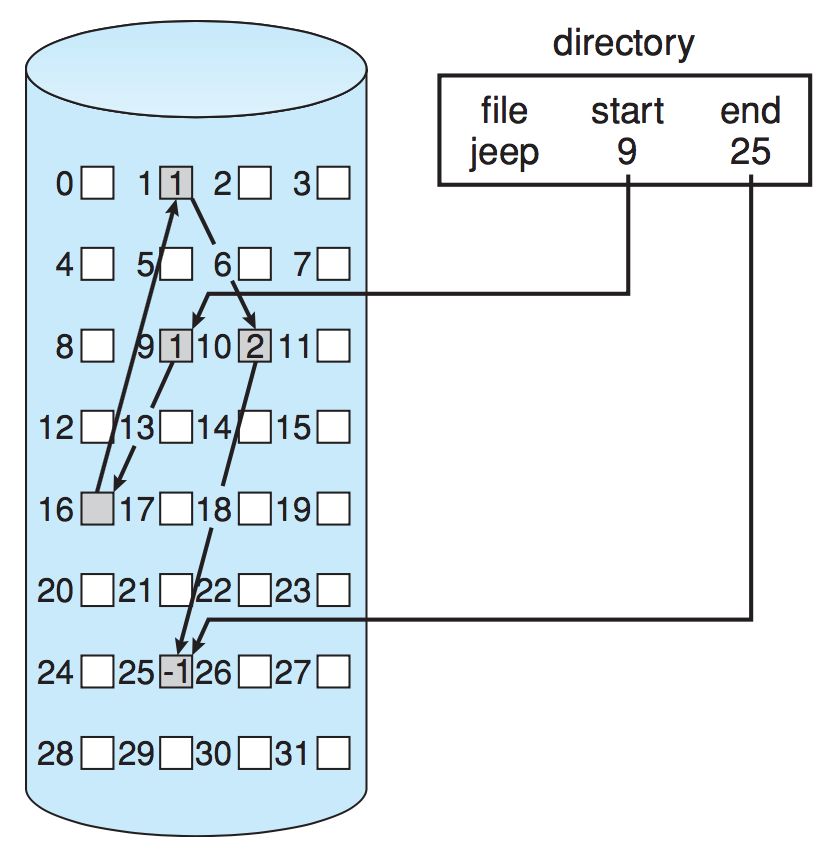
\includegraphics[width=0.6\textwidth]{images/disk-linked.png}
\end{center}

\end{frame}

\begin{frame}
\frametitle{Linked Allocation}

A possible solution to the problem of following so many pointers (and the overhead of maintaining so many) is to group up the blocks into \alert{clusters}.

A cluster is comprised of, say, four blocks. 

Then we waste less memory maintaining pointers and it improves disk accesses because there is less seeking back and forth to various disk locations.

\end{frame}

\begin{frame}
\frametitle{File Allocation Table (FAT)}

One variation of linked allocation is the File Allocation Table (FAT).

Used in Windows before NTFS came in with Windows NT/2000/XP/7/8...

FAT32 hangs on these days for USB Flash Drives.

\end{frame}

\begin{frame}
\frametitle{File Allocation Table}


At the beginning of the disk, there is a table to maintain file allocation data. 

The table has one entry for each block and is indexed by block number. 

It works like a linked list; the directory entry has the first block of the file and the table entry under that block number has the index of the next block. 

The chain continues until the last block; there is a special end-of-file value. 

\end{frame}

\begin{frame}
\frametitle{File Allocation Table}

An unused block has a table value of 0. 

Thus, to allocate a new block, find the first 0-valued entry, and replace the previous end-of-file value with the address of the new block.

\end{frame}

\begin{frame}
\frametitle{File Allocation Table}

\begin{center}
	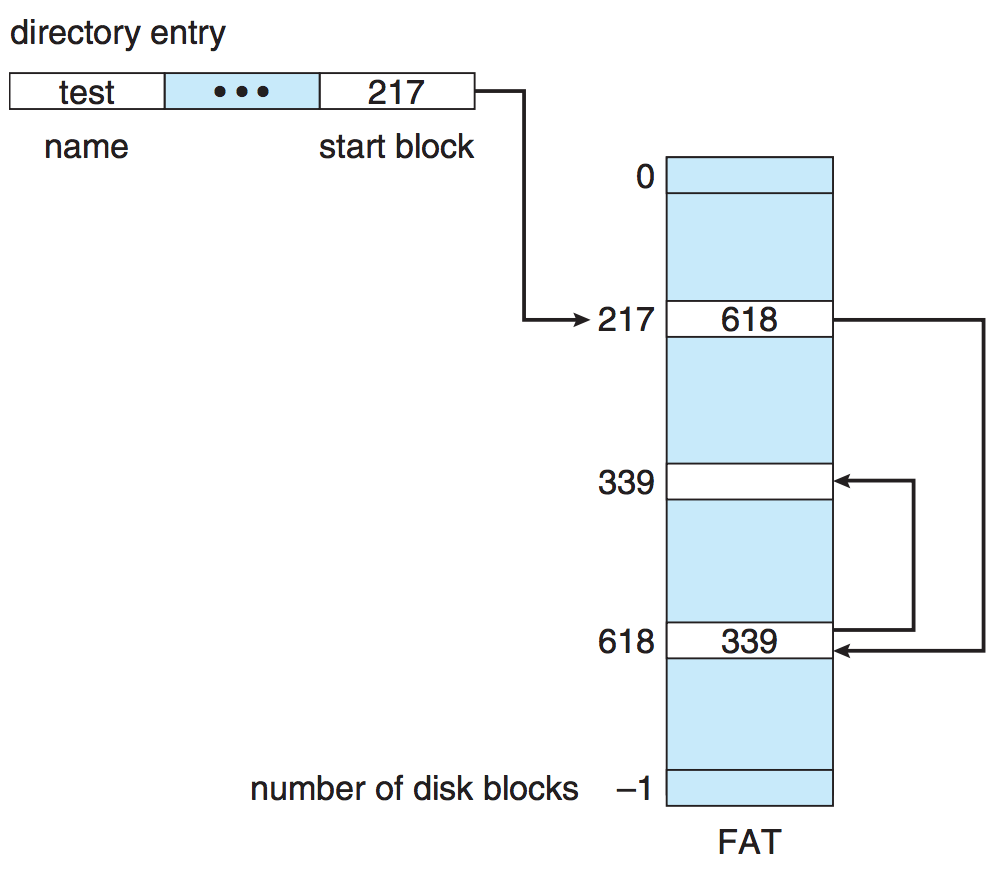
\includegraphics[width=0.6\textwidth]{images/file-allocation-table.png}
\end{center}

The FAT itself should be cached in memory, otherwise the disk is going to have to seek back to it unbearably often.

\end{frame}



\begin{frame}
\frametitle{Indexed Allocation}

If we stuck to pure linked allocation, we still have the problem that accessing some part in the middle of the file is a pain.

We have to follow and retrieve a lot of pointers to the different blocks. 

The idea of indexed allocation is to take all the pointers and put them into one location: an index block. 


\end{frame}



\begin{frame}
\frametitle{Indexed Allocation}

So, the first block of the file contains a whole bunch of pointers. 

To get to block $i$, just go to index $i$ of the index block and we can get the location of block $i$ much more efficiently than we could in linked allocation. 

All pointers to blocks start as null, and when we add a new block, add its corresponding entry into the index block.

\end{frame}

\begin{frame}
\frametitle{Indexed Allocation}

\begin{center}
	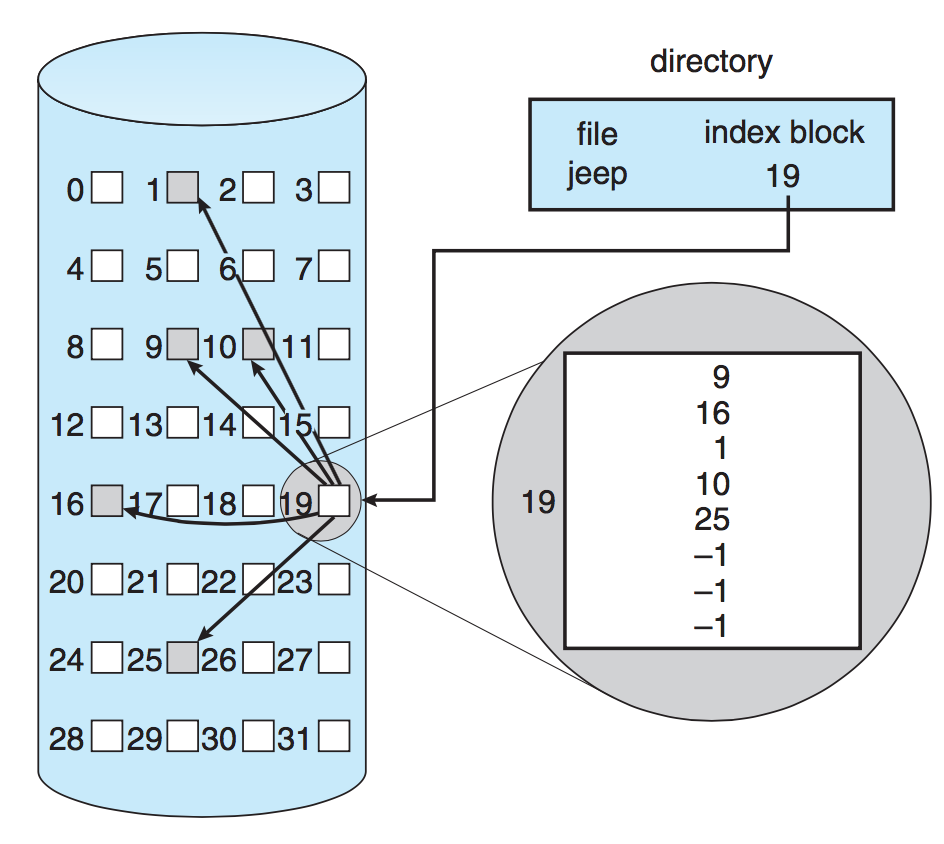
\includegraphics[width=0.6\textwidth]{images/disk-indexed.png}
\end{center}


\end{frame}

\begin{frame}
\frametitle{Block Size}

Like many of the other systems we have examined, there is a need to make a decision about the size of a block. 

If a file needs only 1-2 blocks, one whole block is allocated for the pointers which contains only 1-2 entries. 

That suggests we want the index to be small, but what if we need more pointers than fit into one block? There are a few mechanisms for this.


\end{frame}

\begin{frame}
\frametitle{Block Size}

What if we need more pointers than fit into one block?

\begin{enumerate}
	\item \textbf{Linked Scheme}
	\item \textbf{Multilevel Index}
	\item \textbf{Combined Scheme}
\end{enumerate}


\end{frame}

\begin{frame}
\frametitle{UNIX inodes}

We can finally show a visual representation of an inode.

\begin{center}
	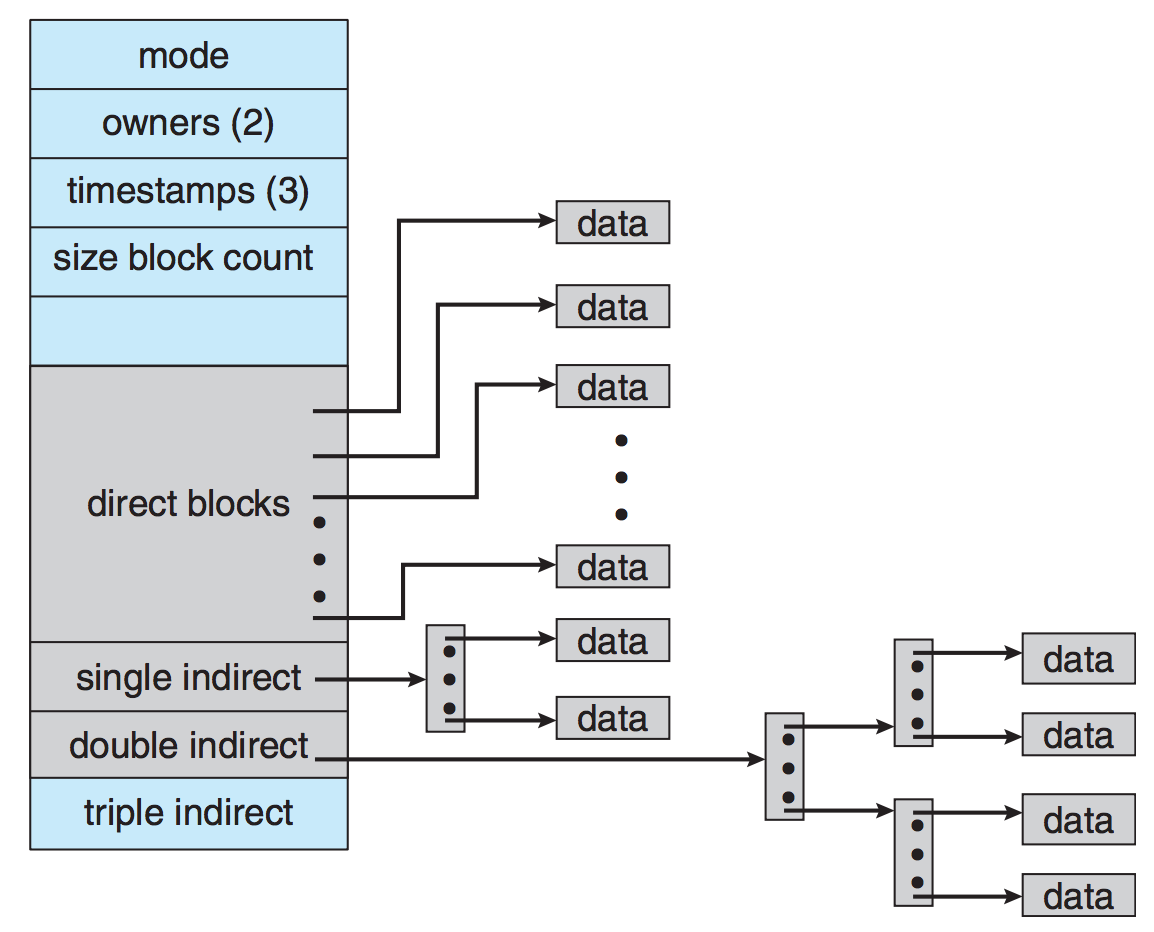
\includegraphics[width=0.6\textwidth]{images/unix-inode.png}
\end{center}
\end{frame}

\begin{frame}
\frametitle{Free Space Management}

As with memory, the system will keep track of the free space available.

Bit vectors work just the way we would expect: create a structure in memory where a bit represents a block. 

If it is free, the bit is 1; allocated is 0. 

So a bit vector looks like \texttt{0100110111011111000000...}. 

The problem with this strategy is, of course, that the bigger the disk, the more overhead is needed to store this bit vector.

\end{frame}

\begin{frame}
\frametitle{Free Space Management}

The next rather obvious approach is a linked list: the head points to the first free space block, and we can traverse the list to get to the next free block. 

\begin{center}
	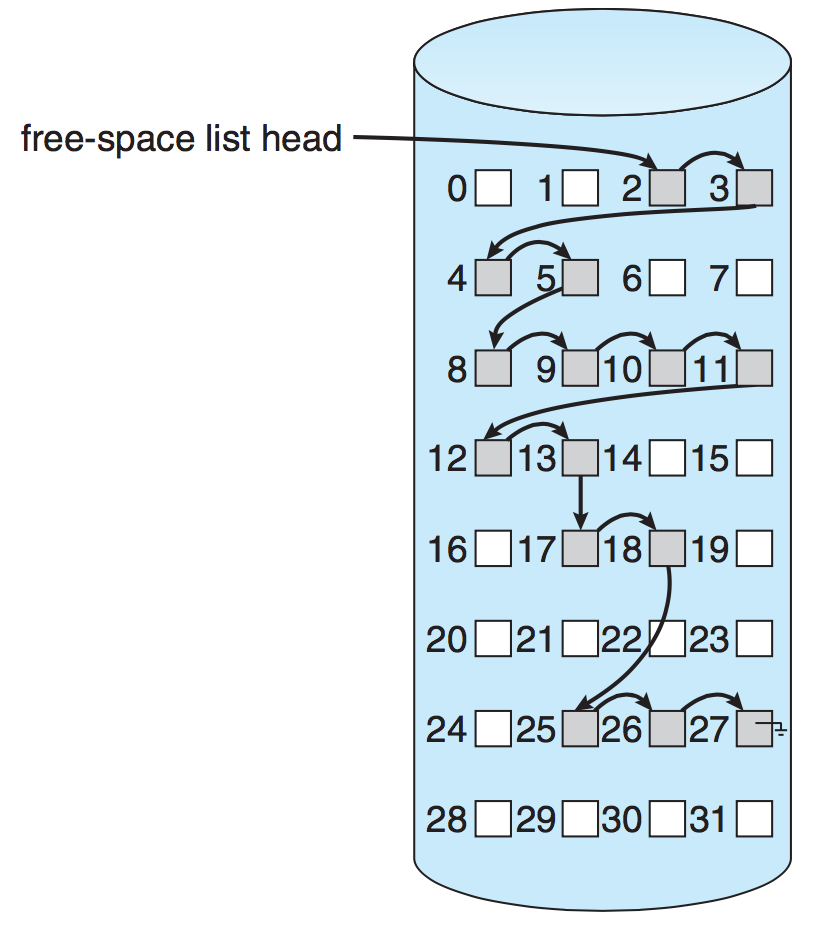
\includegraphics[width=0.4\textwidth]{images/disk-linked-list.png}
\end{center}


\end{frame}

\begin{frame}
\frametitle{Grouping}

Grouping: the first free block will be used to store the addresses of $n$ free blocks, the first $n-1$ of which are actually free. 

The last block contains a block with another set of $n$ free blocks. 

So if we need a large number of free blocks, we can find them quickly, instead of walking through the list one block at a time, which takes a lot of disk accesses. 

\end{frame}

\begin{frame}
\frametitle{Counting}

Counting is a slight improvement on this where we also store a number $k$ of free contiguous blocks after each address. 

So, if block 27 is followed by three consecutive free blocks, instead of having 27, 28, 29, 30 as entries, it will show (27, 4). 

The entries may be stored in a balanced tree for efficient operations.



\end{frame}

\begin{frame}
\frametitle{Preallocation}

The efficient use of a disk depends on the disk-allocation/directory algorithms. 

UNIX inodes, for example, are preallocated, so even a disk containing no files has some of its space taken up by the inodes. 

Preallocation \& distribution of inodes improves the file system performance.

UNIX allocation and free-space algorithms keep the file data near the inode, where possible, to reduce seek time.


\end{frame}


\end{document}

